% !TeX spellcheck = it_IT
\newpage
\section{Agenti risolutori di problemi}
Gli agenti risolutori di problemi adottano il paradigma della risoluzione di problemi come \textbf{ricerca} in uno \textbf{spazio di stati}. Sono agenti con \textbf{modello} (storia percezioni e stati) che adottano una rappresentazione \textbf{atomica} degli stati.\\
Sono particolari gli agenti con \textbf{obiettivo} che pianificano l'intera sequenza di mosse prima di agire.

\subsection{Processo di risoluzione}
I passi da seguire sono i seguenti:
\begin{enumerate}
	\item \textbf{Determinazione di un obiettivo}, ovvero un insieme di stati in cui l'obiettivo è soddisfatto
	\item \textbf{Formulazione} del problema tramite la rappresentazione degli stati e delle azioni
	\item Determinazione della \textbf{soluzione} mediante la ricerca
	\item \textbf{Esecuzione} del piano
\end{enumerate}

\begin{example}[Viaggio con mappa]
	Supponiamo di voler fare un viaggio. Il processo di risoluzione sarebbe il seguente:
	\begin{enumerate}
		\item Raggiungere Bucarest
		\item \begin{itemize}
			\item Azioni: guidare da una città all'altra
			\item Stato: città su mappa
		\end{itemize}
	\end{enumerate}
\end{example}

\subsection{Assunzioni}
Assumiamo che l'ambiente in questione sia \textbf{statico}, \textbf{osservabile}, \textbf{discreto} e \textbf{deterministico} (assumiamo un mondo ideale).

\subsection{Formulazione del problema}
Un problema può essere definito formalmente mediante 5 componenti:
\begin{enumerate}
	\item \textbf{Stato iniziale}
	\item \textbf{Azioni} possibili
	\item \textbf{Modello di transizione}: $ris: stato \times azione \to stato$, uno stato \emph{successore} $ris(s,a)=s'$
	\item \textbf{Test obiettivo} per capire tramite un insieme di stati obiettivo se il goal è raggiunto $test: stato \to \{true,false\}$
	\item \textbf{Costo del cammino}: composto dalla somma dei costi delle azioni, dove un passo ha costo $c(s,a,s')$. Un passo non ha mai costo negativo.
\end{enumerate}
I punti 1, 2 e 3 definiscono implicitamente lo \textbf{spazio degli stati}. Definirlo esplicitamente può essere molto costoso.

\subsection{Algoritmo di ricerca}
Gli algoritmi di ricerca prendono in input un problema e restituiscono un \textbf{cammino soluzione}.\\
Dobbiamo misurare le \textbf{prestazioni}: trova una soluzione? Quanto costa trovarla? Quanto è efficiente?
\begin{equation*}
	costo\_totale=costo\_ricerca+costo\_cammino\_sol
\end{equation*}

\begin{example}[Arrivare a Bucarest]
	Partiamo con la formulazione del problema:
	\begin{enumerate}
		\item \textbf{Stato iniziale}: la città di partenza, ovvero Arad
		\item \textbf{Azioni}: spostarsi in una città collegata vicina
		\begin{lstlisting}
			Azioni(In(Arad))={Go(Sibiu),Go(Zerind),...}
		\end{lstlisting}
		\item \textbf{Modello di transizione}: 
		\begin{lstlisting}
			Risultato(In(Arad), Go(Sibiu)) = In(Sibiu)
		\end{lstlisting}
		\item \textbf{Test obiettivo}:
		\begin{lstlisting}
			{In(Bucarest)}
		\end{lstlisting}
		\item \textbf{Costo del cammino}: somma delle lunghezze delle strade
	\end{enumerate}
	In questo esempio lo spazio degli stati coincide con la rete dei collegamenti tra le città.
	\begin{center}
		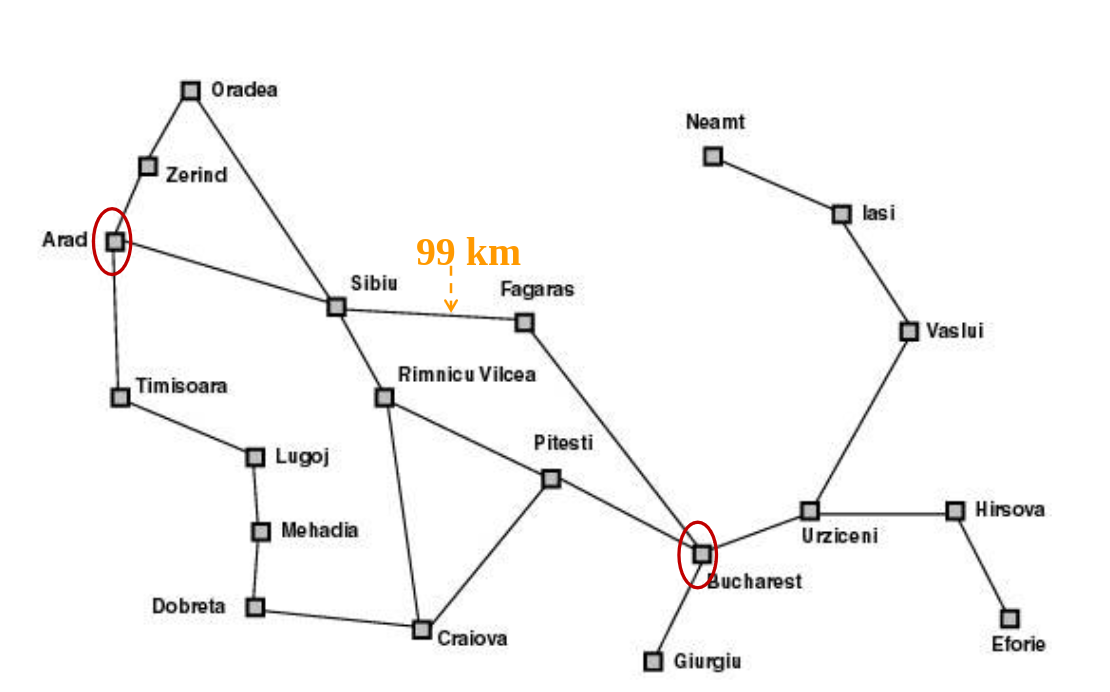
\includegraphics[scale=0.2]{images/bucarest_example.png}
	\end{center}
\end{example}

\begin{example}[Puzzle dell'8]
	Partiamo con la formulazione del problema:
	\begin{enumerate}
		\item \textbf{Stati}: tutte le possibili configurazioni della scacchiera
		\item \textbf{Stato iniziale}: una configurazione tra quelle possibili
		\item \textbf{Obiettivo}: una configurazione del tipo
		\begin{center}
			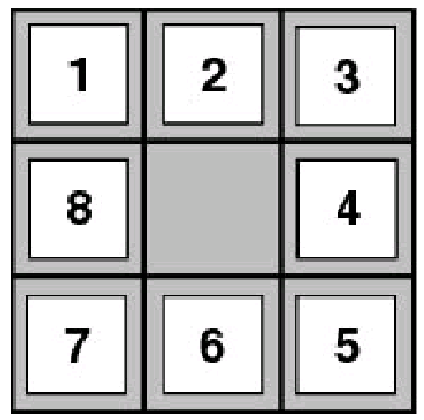
\includegraphics[scale=0.2]{images/8_puzzle_win.png}
		\end{center}
		\item \textbf{Azioni}: le mosse della casella vuota
		\item \textbf{Costo cammino}: ogni passo costa 1
	\end{enumerate}
	In questo esempio lo spazio degli stati è un grafo con possibili cicli (ci possiamo ritrovare in configurazioni già viste). Il problema è NP-completo: per 8 tasselli ci sono $\frac{9!}{2}=181.000$ stati.
\end{example}

\begin{example}[8 regine]
	Supponiamo di dover collocare 8 regine su una scacchiera in modo tale che nessuna regina sia attaccata da altre.
	\begin{enumerate}
		\item \textbf{Stati}: tutte le possibili configurazioni della scacchiera con 0-8 regine
		\item \textbf{Goal test}: avere 8 regine sulla scacchiera, di cui nessuna è attaccata
		\item \textbf{Azioni}: aggiungi una regina
	\end{enumerate}
	In questo esempio lo spazio degli stati sono le possibili scacchiere, ovvero $64 \times 63 \times \ldots \times 57 \simeq 1.8 \times 10^{14}$.\\
	Proviamo ad utilizzare una formulazione diversa:
	\begin{enumerate}
		\item \textbf{Stati}: tutte le possibili configurazioni della scacchiera in cui \emph{nessuna regina è minacciata}
		\item \textbf{Goal test}: avere 8 regine sulla scacchiera, di cui nessuna è attaccata
		\item \textbf{Azioni}: aggiungere una regina nella colonna vuota più a destra ancora libera in modo che non sia minacciata
	\end{enumerate}
	Lo spazio degli stati passa a $2057$, anche se comunque rimane esponenziale per $k$ regine.\\
	Vediamo infine un'ultima formulazione:
	\begin{enumerate}
		\item \textbf{Stati}: scacchiere con 8 regine, una per colonna
		\item \textbf{Goal test}: nessuna delle regine già presenti è attaccata
		\item \textbf{Azioni}: sposta una regina nella colonna se minacciata
		\item \textbf{Costo cammino}: zero
	\end{enumerate}
	Qui lo spazio degli stati è di qualche decina di milione.\\
	Capiamo quindi che formulazioni diverse del problema portano a spazi di stati di dimensioni diverse.
\end{example}

\begin{example}[Dimostrazione di teoremi]
	Dato un insieme di premesse:
	\begin{equation}
		\{s, t, q \Rightarrow p, r \Rightarrow p, v \Rightarrow q, t \Rightarrow r, s \Rightarrow v\}
	\end{equation}
	dimostrare una proposizione $p$ utilizzando solamente la regola di inferenza \emph{Modus Ponens}:
	\begin{equation*}
		(p \wedge p\Rightarrow q) \Rightarrow q
	\end{equation*}
	Scriviamo la formulazione del problema:
	\begin{itemize}
		\item \textbf{Stati}: insieme di proposizioni
		\item \textbf{Stato iniziale}: le premesse
		\item \textbf{Stato obiettivo}: un insieme di proposizioni contenente il teorema da dimostrare
		\item \textbf{Operatori}: l'applicazione del Modus Ponens
	\end{itemize}
	Lo spazio degli stati è quindi il seguente:
	\begin{center}
		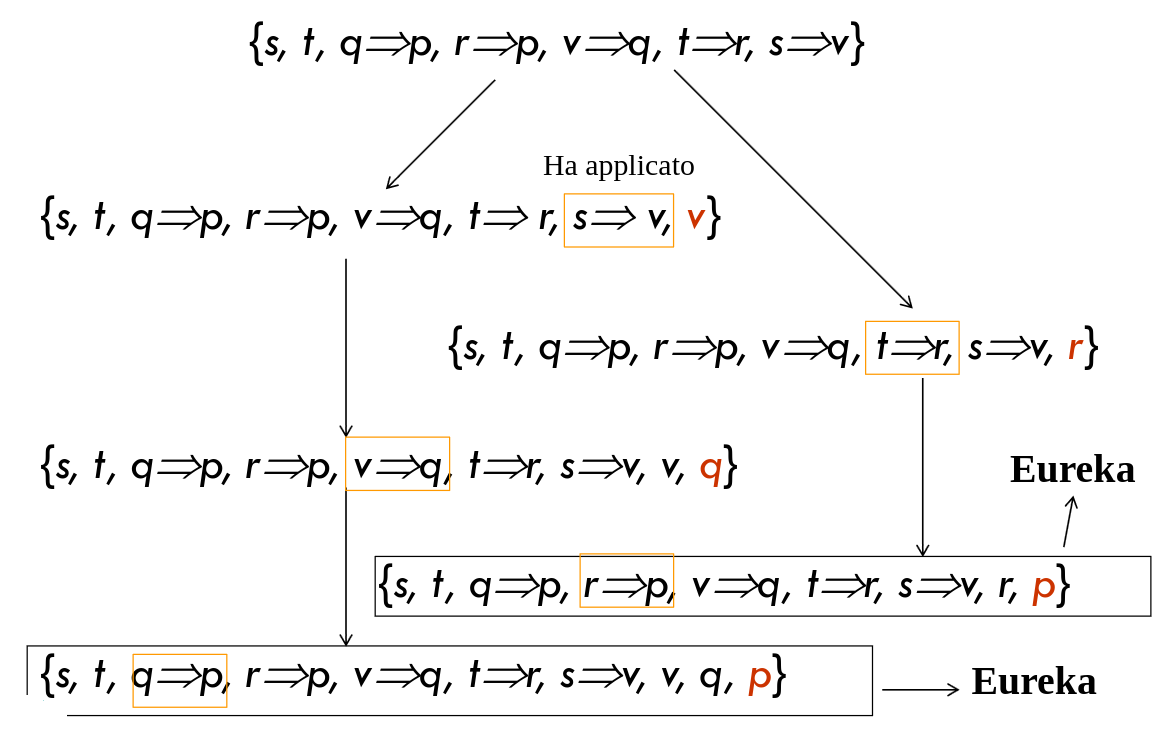
\includegraphics[scale=0.3]{images/dimostrazione_teoremi.png}
	\end{center}
\end{example}

\subsection{Ricerca della soluzione}
La ricerca della soluzione consiste nella generazione di un \textbf{albero di ricerca} a partire dalle possibili sequenze di azioni che si sovrappone allo spazio degli stati.\\
Ad esempio per il caso di Bucarest:
\begin{center}
	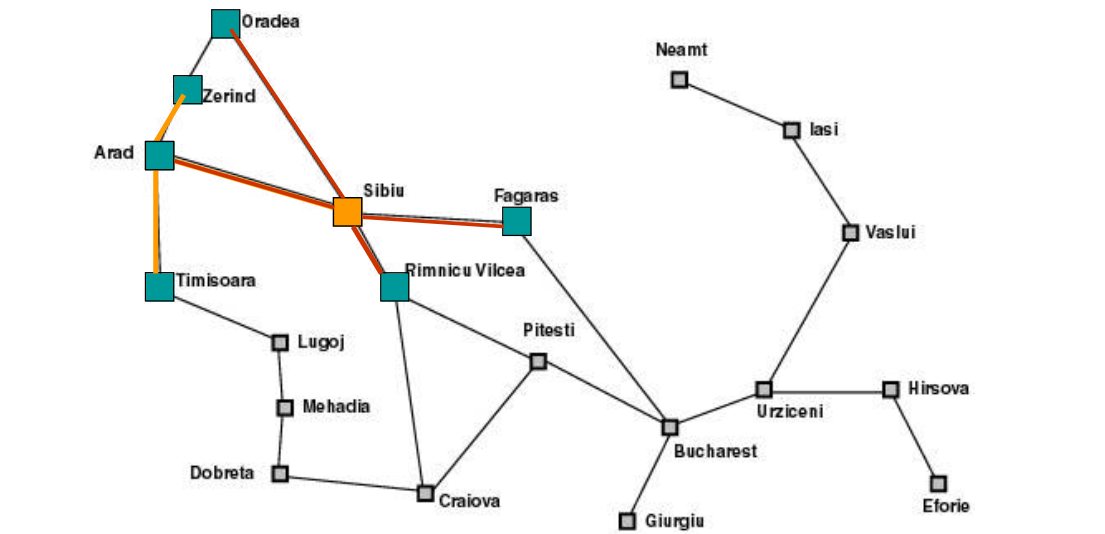
\includegraphics[scale=0.3]{images/bucarest_tree.png}
\end{center}
Espandiamo ogni nodo con i suoi possibili successori (frontiera).
\begin{observation}
	Si noti che un nodo dell'albero è diverso da uno stato. Infatti possono esitere nodi dell'albero di ricerca con lo stesso stato (si può tornare indietro).
\end{observation}